\documentclass[]{beamer}
\usepackage{framed}
%to include graphics
\usepackage{graphicx}
%to include code
\usepackage{listings}
\usepackage{courier}
%to include hyperlinks
\usepackage{hyperref}
\usepackage{caption}
\usepackage{pifont}
%used for amsfonts
\usepackage{amsmath}
%used for mathscr
\usepackage{mathrsfs}
%used for indicator function (mathbbm)
\usepackage{dsfont}
%no page numbering
%\usepackage{nopageno}
%used for aligning graphics
%\usepackage{adjustbox}

\lstset{
         basicstyle=\tiny\ttfamily, 	% Standardschrift
         %numbers=left,     			% Ort der Zeilennummern
         numberstyle=\tiny,          % Stil der Zeilennummern
         %stepnumber=2,              % Abstand zwischen den Zeilennummern
         numbersep=5pt,              % Abstand der Nummern zum Text
         tabsize=2,                  % Groesse von Tabs
         extendedchars=true,         %
         breaklines=true,            % Zeilen werden Umgebrochen
         keywordstyle=\color{red},
    		frame=b,         
 %        keywordstyle=[1]\textbf,    % Stil der Keywords
 %        keywordstyle=[2]\textbf,    %
 %        keywordstyle=[3]\textbf,    %
 %        keywordstyle=[4]\textbf,   \sqrt{\sqrt{}} %
         stringstyle=\color{white}\ttfamily, % Farbe der String
         showspaces=false,           % Leerzeichen anzeigen ?
         showtabs=false,             % Tabs anzeigen ?
         xleftmargin=17pt,
         framexleftmargin=17pt,
         framexrightmargin=5pt,
         framexbottommargin=4pt,
         %backgroundcolor=\color{lightgray},
         showstringspaces=false      % Leerzeichen in Strings anzeigen ?        
 }
 
\linespread{1.3}


\DeclareCaptionFont{white}{\color{white}}
\DeclareCaptionFormat{listing}{\colorbox[cmyk]{0.43, 0.35, 0.35,0.01}{\parbox{\textwidth}{\hspace{15pt}#1#2#3}}}
\captionsetup[lstlisting]{format=listing,labelfont=white,textfont=white, singlelinecheck=false, margin=0pt, font={bf,footnotesize}}


%for beamer theme
\usetheme[pageofpages=of,% String used between the current page and the
                         % total page count.
          bullet=circle,% Use circles instead of squares for bullets.
          titleline=true,% Show a line below the frame title.
          alternativetitlepage=true,% Use the fancy title page.
          ]{Torino}

\setbeamercovered{invisible}          
\setbeamertemplate{section page}
{
	\huge{\insertsection}
	 \textcolor{chameleongreen3}{\hrule height 1pt} 	
  	\vspace{0px}
}  

\newcommand{\hiddencell}[2]{\action<#1->{#2}}
% first argument: slide number to appear from, second argument: content of cell        

%-----------------------------------------------------------
%-----------------------------------------------------------
%-----------------------------------------------------------
%-----------------------------------------------------------

\author[Johanning]{Simon Johanning}
\title{Early gene regulation of osteogenesis in embryonic stem cells}
\institute{Institut f\"ur Mathematik und Informatik der Universit\"at Leipzig}

\pagestyle{plain}
\AtBeginSection{\frame{\sectionpage}}



\begin{document}	
\watermarkoff



\begin{frame}[t,plain]
	\titlepage
\end{frame}

\pagenumbering{gobble}

\section{Hintergrund}

\begin{frame}{Wissenschaftlicher Hintergrund}
\begin{itemize}
	\item Signal pathways und Ver\"anderung der Genexpression von Stammzellendifferentiation von M\"ausen (mES) nicht gut charakterisiert
	\pause
	\item Differenzierung in pluripotente Zellen in Knochengewebe essentiell f\"ur therapeutische Anwendungen (insbesondere tissue engineering)
	\pause
	\item Genregulatorische Netzwerke nicht klar
\end{itemize}
\end{frame}

\begin{frame}{Biologischer Hintergrund: Gene / TFs}
\begin{itemize}
	\item Runx2 wesentliches regulatorisches Gen in Osteoblasten
	\pause
	\\ Wichtig f\"ur (down-stream) Expression vieler osteogenetischer Gene
	\pause
	\item Bekannt, dass von Wachstumsfaktoren BMP2 und TGF$\beta$1 reguliert
	\pause
	\item Ebenso von Genen Dlx5 und Msx2, welche beide von BMP2 und TGF$\beta$1 beeinflusst werden
	\pause	
	\item Dlx5 von BMP2 allein stimuliert
	\pause
	\item Msx2 wird oft als negativer Regulator von Runx2 gesehen
	\pause
	\\ Aber: Rolle nicht klar; Manche Studien: Msx2 supprimiert, manche kein Effekt, manche pro-osteogenetisch unabh\"angig von Runx2
\end{itemize}
\end{frame}

\begin{frame}{Biologischer Hintergrund: Wachstumsfaktoren}
\begin{itemize}
	\item Wichtige Wachstumsfaktoren O.: BMP2 (\emph{Bone Morphogenetic Protein 2}) und TGF$\beta$1 (\emph{Transforming Growth Factor $\beta$1})
	\pause
	\item BMP2: positiver Regulator in Osteogenese
	\pause
	\item TGF$\beta$1: negativer Regulator in O.; hohe Konzentration in Knochen und Knorpelgewebe
	\pause
	\item Aber: Manche Studien sehen TGF$\beta$1 als pro-osteogenisch, (manche als kontra-osteogenisch)
	\pause
	\item osteog. Rolle von TGF$\beta$1 h\"angt von Zelltyp und Umgebung ab
	\pause
	\item wenige \emph{in vitro}-Studien, die TGF$\beta$1 und BMP2 untersuchen
\end{itemize}
\end{frame}

\begin{frame}{Biologischer Hintergrund: Motivation}
\begin{itemize}
	\item Signal- und Regulationsnetzwerke, die Interaktion zwischen BMP2 und TGF$\beta$1 regeln, sind nicht bekannt
	\pause
	\item Kandidaten f\"ur GRN: Dlx5 und Msx2, da diese um Runx2-Promoter konkurrieren
	\pause
	\\ $\rightarrow$ Motivation f\"ur Netzwerke, die BMP2, TGF$\beta$1, Dlx5, Msx2 und Runx2 beinhalten
\end{itemize}
\end{frame}

\begin{frame}{Mathematischer Hintergrund: Boolsche Modelle}
\begin{itemize}
	\item Rigorose Repr\"asentation qualitativen biologischen Wissens
	\pause
	\item Komponenten (\emph{Spezies}) haben diskrete Zust\"ande; oftmals bin\"ar: \emph{An/Aus}
	\pause
	\item Repr\"asentation als Graphen: Gene/Faktoren als Knoten, Interaktionen als Kanten (aktivierend/inhibierend)
	\pause
	\item Diskrete Zeit: Zustand(t+1) h\"angt von Zust\"anden(t) ab
	\pause
	\item stabile steady-states: Zellph\"anotypen, die mit experimentellen Daten verglichen werden k\"onnen
	\pause
	\item Auch wenn grob, k\"onnen BM das qualitative Verhalten biologischer Systeme recht gut reproduzieren
\end{itemize}
\end{frame}

\begin{frame}{Boolsche Modelle: Beschr\"ankungen}
\begin{itemize}
	\item K\"onnen weder kontinuierliche Konzentrationslevel noch realistische Zeitskalen abbilden
	\pause
	\\ $\Rightarrow$ K\"onnen quantitative (biologische) Experimente weder erkl\"aren noch vorhersagen
	\pause (zunehmend wichtig in systems biology)
	\\ \pause $\rightarrow$ \"Ubergang zu Differentialgleichungssystemen: HillCube Methode / odefy
\end{itemize}
\end{frame}

\section{Forschungsansatz}

\begin{frame}{Setup Studie (grob)}
\begin{itemize}
	\item Messung Genexpression von Runx2, Dlx5 und Msx2 unter Zugabe von TFs BMP2, TGF$\beta$1 und Kombination
	\pause
	\item Konstruktion Boolscher Modelle
	\pause
	\item \"Uberf\"uhrung in HillCube-Modelle (DGLs)
	\pause
	\item Rekonstruktion der experimentellen Daten mittels HillCube-Modelle
	\pause
	\item Testen der Vorhersagen der Modelle mit experimentellen Daten mittel \"Uber- und Unterexpression
	\pause
	\\ $\rightarrow$ Reduktion der m\"oglichen Modelle ($3^{5} \rightarrow 1$)
\end{itemize}
\end{frame}

\begin{frame}{Genexpression bzgl. WF}
\begin{itemize}
	\item Zugabe von BMP2, TGF$\beta$1, sowie Kombination in embryonische Stammzellenkultur
	\pause
	\item Messung der Expression von Runx2, Dlx5 und Msx2, normalisiert an Kontrollgruppe (ohne Zugabe von Wachstumsfaktoren) an $t \in \{0,8,16,24(,48)\}$
	\pause
	\item System steady-state an t=24h; t=48h ver\"andert System nicht signifikant
\end{itemize}
\end{frame}

\begin{frame}{Boolsche Modelle: Kandidatennetzwerke}
Modellierung Genregulationsnetzwerk nach Literatur:
	\pause
	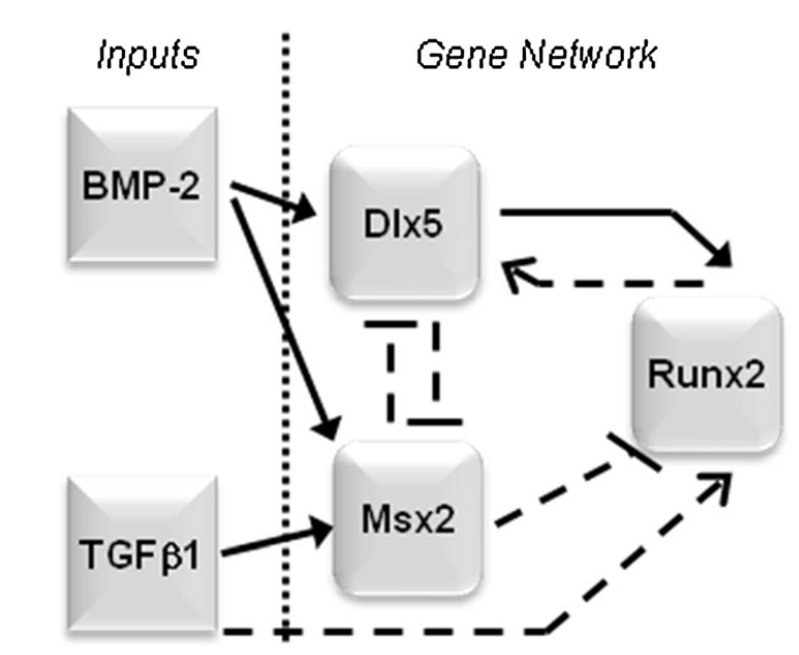
\includegraphics[scale=0.22]{regulatory_network.jpg}
	\pause
\end{frame}

\begin{frame}{Genexpression bzgl. WF: Ergebnis}
\begin{center}
			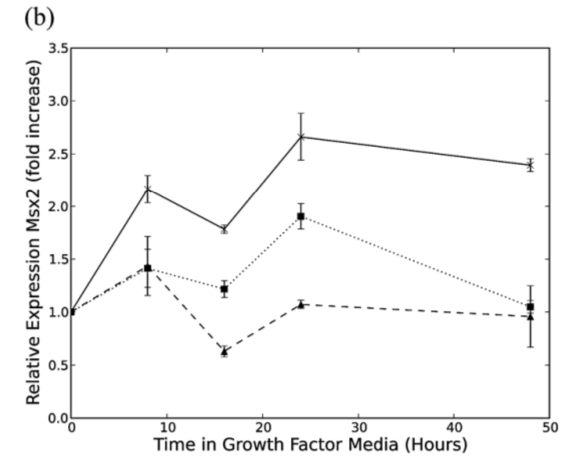
\includegraphics[scale=0.18]{Expression_Msx2.jpg}
			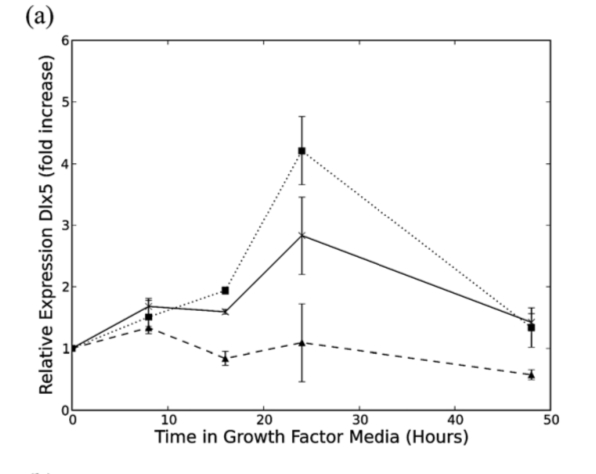
\includegraphics[scale=0.18]{Expression_Dlx5.jpg}
			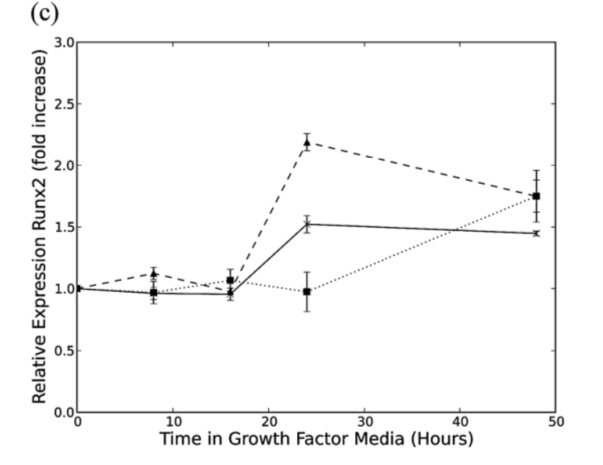
\includegraphics[scale=0.18]{Expression_Runx2.jpg}
	\\------ BMP2 - - - TGF$\beta$1 ...... BMP2/TGF$\beta$1
\end{center}
\end{frame}

\begin{frame}{Vergleich Expressionsprofile mit bin\"aren Daten}
Vergleich Kandidatennetzwerke mit Expressionsdaten an t=24:
\pause
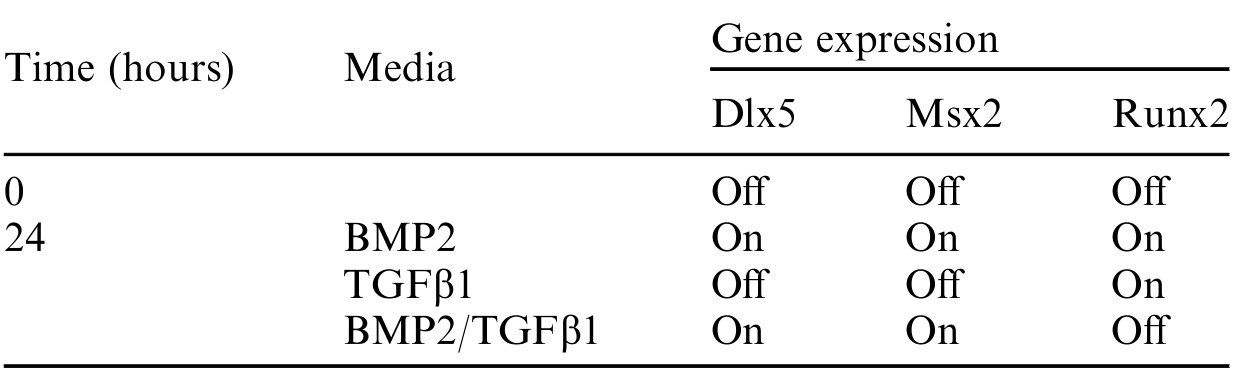
\includegraphics[scale=0.25]{table1.jpg}
\pause
	\\ Daten Input in BM
\end{frame}

\begin{frame}{odefy}
\begin{itemize}
	\item Problem BM: weder kontinuierliche Konzentrationslevel noch realistische Zeitskalen
	\pause
	\item ODEs: Erlauben detailliertere und quantitative Charakterisierung der Genregulationsnetzwerke
	\pause
	\item stabile steady-states in ODEs: Zellph\"anotypen
\end{itemize}
\end{frame}

\begin{frame}{odefy}
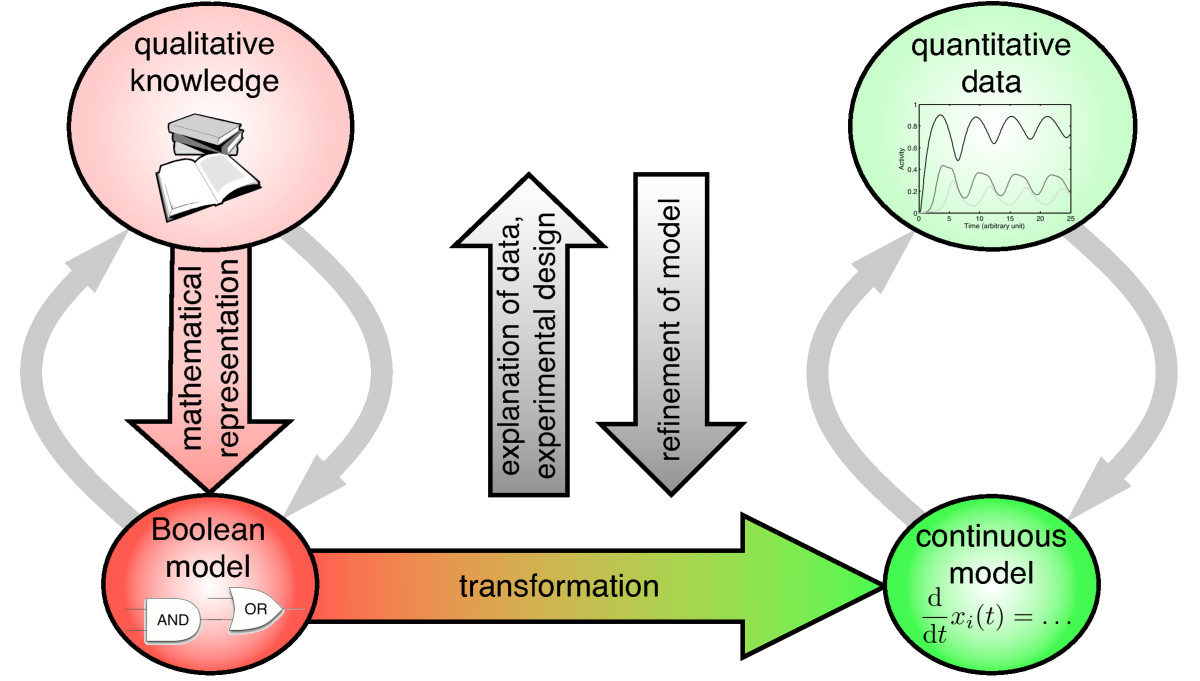
\includegraphics[scale=0.8]{odefy.jpg}
\end{frame}

\begin{frame}{HillCube-Modell}
$\overline{B_{i}}$ HillCube-Modell von $\overline{x_{i}}$; 
	\pause
	\\ Differentialgleichung $\dot{\overline{x_{i}}} = \frac{1}{\tau_{i}} (\overline{B_{i}}(\overline{x}_{i_{1}},\overline{x}_{i_{2}},...,\overline{x}_{i_{N_{i}}}) - \overline{x_{i}})$
	\\ mit $\tau_{i}$ Lebensdauer der Spezies $X_{i}$
\end{frame}

\begin{frame}{Expressionsprofile}
\begin{center}
			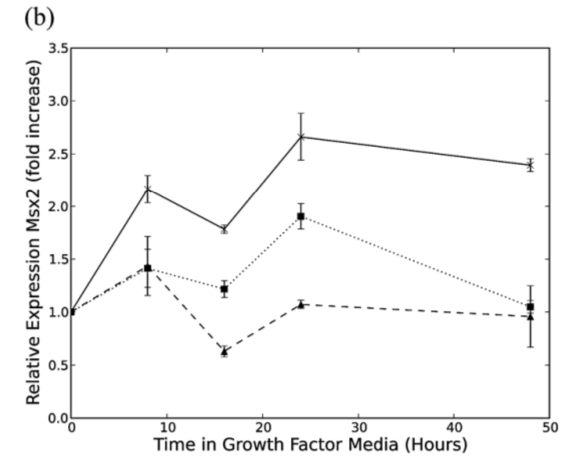
\includegraphics[scale=0.18]{Expression_Msx2.jpg}
			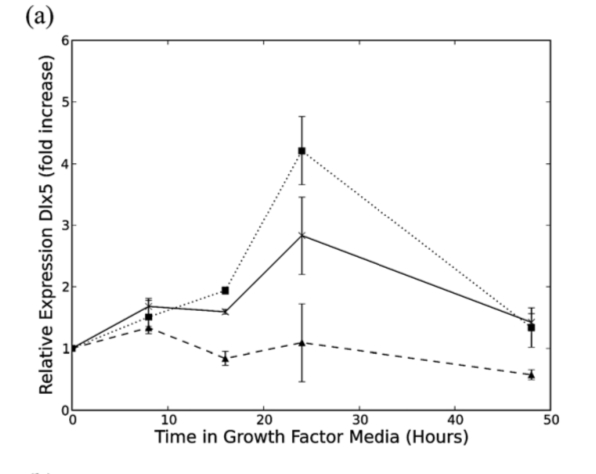
\includegraphics[scale=0.18]{Expression_Dlx5.jpg}
			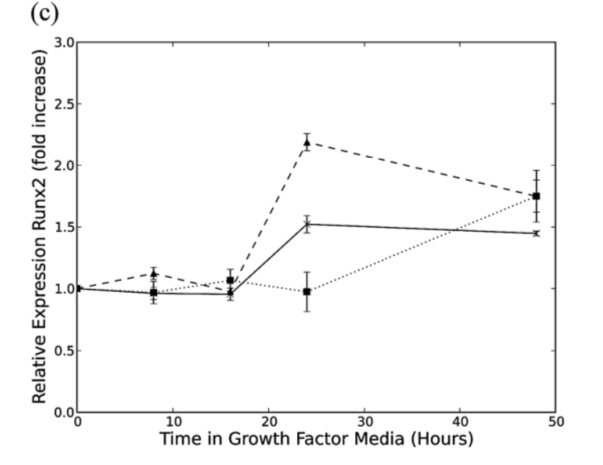
\includegraphics[scale=0.18]{Expression_Runx2.jpg}
	\\------ BMP2 - - - TGF$\beta$1 ...... BMP2/TGF$\beta$1
\end{center}
\end{frame}

\begin{frame}{Reduzierte Kandidatennetzwerke}
Modelle, die Verhalten reproduzieren:
	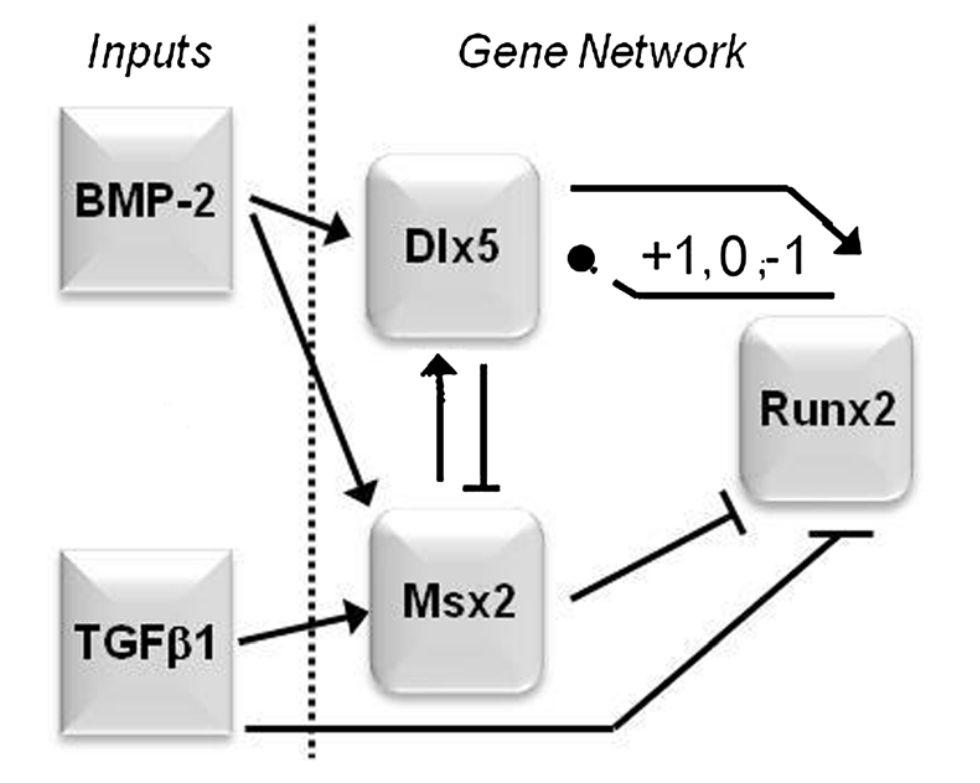
\includegraphics[scale=0.22]{regulatory_network_results.jpg}
\end{frame}

\begin{frame}{Testen Vorhersage \"Uber- und Unterproduktion}
\begin{itemize}
	\item Vorhersage Verhalten bei \"Uber und Unterproduktion von TFs (Var. $\in \{0,1\}$)
	\pause
	\item Vorhersage steady-state Dlx5, Msx2; Verhalten von Runx2 unklar
	\pause
	\item Runx2 reguliert Dlx5 positiv: up-regulation in TGF$\beta$1 und Kontrollmedium; down-regulation von Msx2 in TGF$\beta$1
	\pause
	\item Ansonsten down-regulation von Dlx5 in TGF$\beta$1 und Kontrollmedium; up-regulation von Msx2 in TGF$\beta$1
	\pause
	\item Vergleichen Vorhersage mit Daten wenn Runx2 \"uberexprimiert
	\pause
	\item Ergebnis Experiment: BM Oszillation in TGF$\beta$1
	\pause
	\\ ODE-modell: Stabile Oszillation nur wenn Runx2 Dlx5 neg. reg.
\end{itemize}
\end{frame}

\begin{frame}{Oszillationen}
\begin{center}
	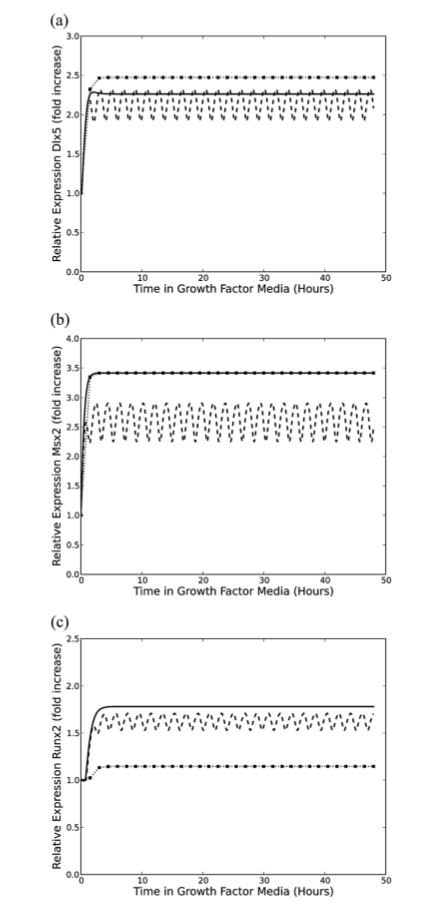
\includegraphics[scale=0.20]{oscillations.jpg}
\end{center}
\end{frame}

\begin{frame}{Zusammenfassung}
\begin{itemize}
	\item Biologisches Wissen f\"ur Konstruktion von Kandidatennetzwerken (BM)
	\pause
	\item Vergleich mit experimentellen Daten: Reduktion auf 3 GRNs
	\pause
	\item \"Uberf\"uhrung in ODEs, Vergleich mit experimentellen Daten: Reduktion auf 1
\end{itemize}
\end{frame}

\section{Kritik}

\begin{frame}{Kritik Setup Studie}
\begin{itemize}
	\item Rolle von TGF$\beta$1 in Osteogenese h\"angt von Zelltyp und lokaler Umgebung ab
	\\ Zelltyp und lokale Umgebung spielen keine Rolle in Studie
	\pause
	\item Keine (kritische) Reflexion welche GRNs betrachtet werden
\end{itemize}
\end{frame}

\begin{frame}{Kritik Interpretation Daten}
	Expression an t=48 nicht auf baseline zur\"uckgekehrt (oder stabil) f\"ur Runx2 und Msx2:
	\\
\begin{center}
			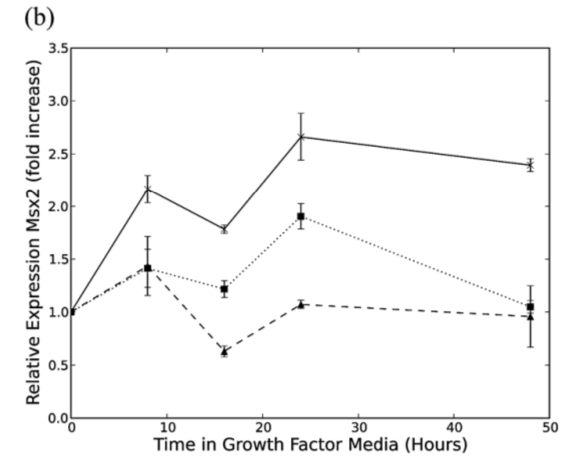
\includegraphics[scale=0.18]{Expression_Msx2.jpg}
			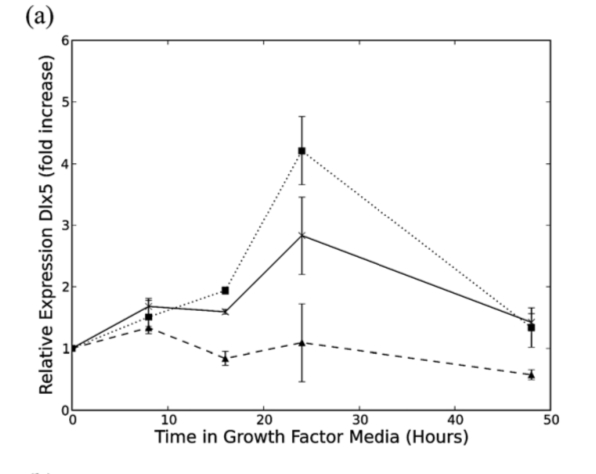
\includegraphics[scale=0.18]{Expression_Dlx5.jpg}
			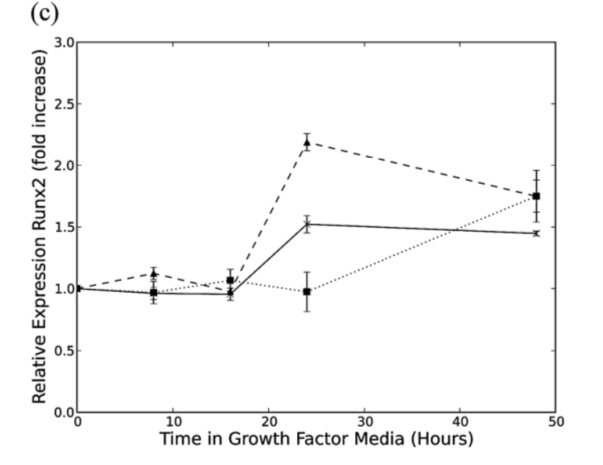
\includegraphics[scale=0.18]{Expression_Runx2.jpg}
	\\------ BMP2 - - - TGF$\beta$1 ...... BMP2/TGF$\beta$1
\end{center}
\end{frame}

\begin{frame}{Kritik Setup boolsches Netzwerk}
\begin{itemize}
	\item Wird gesagt, dass BMP2 Runx2 moderiert, TGF$\beta$1 Dlx5 supprimiert, aber Einfluss von BMP2 auf Runx2, sowie TGF$\beta$1 auf Dlx5 nicht modelliert
\end{itemize}
\end{frame}

\begin{frame}{Kritik Setup boolsches Netzwerk}
		 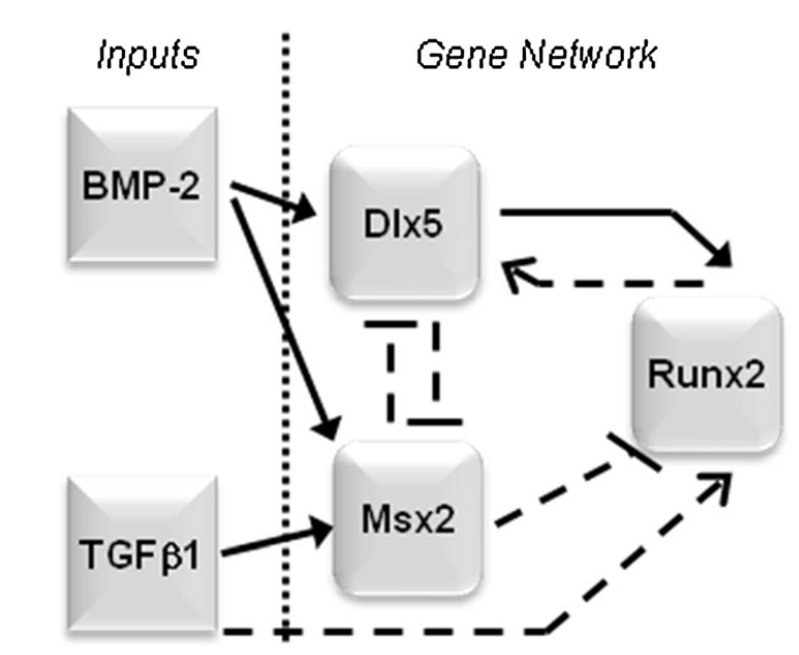
\includegraphics[scale=0.22]{regulatory_network.jpg}
\end{frame}

\begin{frame}{Kritik Setup boolsches Netzwerk}
\begin{itemize}
	\item Wird gesagt, dass BMP2 Runx2 moderiert, TGF$\beta$1 Dlx5 supprimiert, aber Einfluss von BMP2 auf Runx2, sowie TGF$\beta$1 auf Dlx5 nicht modelliert
\pause
\\ Sinnvoll 0 Studien als keinen Einfluss, 1 Studie ungesichert, 2 Studien gesichert?
\pause
\item Ebenfalls: Kein Unterschied ob kein Einfluss oder keine Studien (bekannt)
\end{itemize}
\end{frame}

\begin{frame}{Kritik Aufbau paper}
\begin{itemize}
	\item Mehr Hintergrund und Umsetzung \"uber HillCube n\"otig gewesen
	\pause
	\item Teil der \"Uber- / Unterexpression methodisch nicht sehr deutlich
	\pause
	\item Schlussfolgerungen / Ergebnisse und Methoden vermischt
	\\ (k\"onnte systematischer aufgebaut sein)
	\pause
	\item Diskussion und Schlussfolgerung: bereits in Methodik dargestellt
\end{itemize}
\end{frame}

\begin{frame}{Kritik theoretischer Mehrwert}
\begin{itemize}
	\item Spezielles GRN gew\"ahlt; Keine Diskussion ob andere GRN passend (nicht ausreichend begr\"undet)
	\pause
	\item Allgemeine Betrachtung fehlt: Wann funktioniert Methode, wann nicht?
	\pause
	\\ Wie gross darf ein GRN werden?
	\pause
	Unterschied Gene / WFs?
	\pause
	\\ Welche topologischen / biologischen Eigenschaften muss es aufweisen?
	\pause
	\\ Welche Szenarios k\"onnen gew\"ahlt werden um GRNs zu reduzieren (wie \"Uber- / Unterexpression)?
\end{itemize}
\end{frame}

\begin{frame}{Selbstkritik}
\begin{itemize}
	\item Einzige Selbstkritik: Viele signal processes und Geninteraktionen (die Osteogenese beeinflussen) nicht modelliert
	\pause
	\\ Mehr Daten werden das Problem l\"osen
	\pause
	\\ Selbstaussage paper: Methodik kann auf jedes GRN angewendet werden
\end{itemize}
\end{frame}

\section{Praktikumsarbeit}

\begin{frame}{Optimaler Fall}
Nachvollziehen der Studie:
\begin{itemize}
	\item Hernahme von Expressionsdaten verschiedener Gene in verschiedenen Medien
	\pause
	\item Konstruktion Boolsches Modell / HillCube Modell
	\pause
	\item Reduktion Kandidatennetzwerke
\end{itemize}
\end{frame}

\begin{frame}{Realistischer Fall}
\begin{itemize}
	\item Vermutlich schwer (gute) Genexpressionsdaten f\"ur geeignete (hinreichend kleine) Netzwerke zu finden (Ideen?)
	\pause
	\\ $\rightarrow$ Extraktion der 45 Datenpunkte aus paper (nachbauen)
	\pause
	\item Konstruktion HillCube Modelle mittels odefy
	\pause
	\\ Ausarbeitung der Mathematik
	\pause
	\\ $\rightarrow$ mathematischer Fokus
	\pause
	\\ Auch sinnvoll, da im paper vernachl\"assigt
	\pause
	\item Nachmodellieren des Oszillationsverhaltens bei \"Uber- / Unterexpression
	\pause
	\\ Potentiell problematisch; Kann die Sensitivit\"at nicht einsch\"atzen
\end{itemize}
\end{frame}

\section{Appendix}

\begin{frame}{Formale Darstellung boolsches Modell}
\begin{itemize}
	\item $N$ Spezies $X_{1}, X_{2},..., X_{N}$ mit $x_{i} \in \{0,1\}$
	\pause
	\item F\"ur jede Spezies: Menge von Spezies, die $x_{i}$ beeinflussen: $R_{i} := \{X_{i_{1}},X_{i_{2}}, ...,  X_{i_{N_{i}}}\} \subset \{X_{1},...,X_{N}\}$
	\pause
	, \\ sowie eine Aktualisierungsfunktion $B_{i}: \{0,1\}^{N_{i}} \to \{0,1\}$ f\"ur jede Kombination von $(x_{i_{1}}, ..., x_{i_{2}}, x_{i_{N_{i}}}) \in \{0,1\}^{N_{i}}$
	\pause
	\item Betrachte $B_{i}$ auf (Hyper-)Einheitsw\"urfel: Knoten $(\xi_{i_{1}}, ..., \xi_{i_{2}}, \xi_{i_{N_{i}}}) \in \{0,1\}^{N_{i}}$ entspricht $(\bigwedge_{ij | \xi_{ij} = 1} x_{ij}) \wedge (\bigwedge_{ij | \xi_{ij} = 0} \neg x_{ij}) $
\end{itemize}
\end{frame}

\begin{frame}{Formale Darstellung boolsches Modell}
\begin{itemize}
	\item sum-of-product Repr\"asentation: $B(x_{i_{1}}, ..., x_{i_{2}}, x_{i_{N_{i}}}) = \bigvee_{(\xi_{i_{1}}, ..., \xi_{i_{2}}, \xi_{i_{N_{i}}}) | B_{i}(\xi_{i_{1}}, ..., \xi_{i_{2}}, \xi_{i_{N_{i}}})=1 } [(\bigwedge_{ij | \xi{ij} = 1} x_{ij}) \wedge (\bigwedge_{ij | \xi{ij} = 0} \neg x_{ij})] $
	\pause
	\item Nun ersetzen von $x_{i} \in \{0,1\}$ durch $\overline{x_{i}} \in [0,1] \rightarrow \overline{B_{i}}: [0,1]^{n} \to [0,1]$: kontinuierliche homologe von $B_{i}$
	\pause
	\item Normalisierte HillCubes: $\overline{B}^{H}_{n_{i}}(\overline{x_{1}}, \overline{x_{2}},...,\overline{x_{n}}) := \overline{B}^{I}_{i}(\frac{f_{i_{1}}(\overline{x_{i_{1}}})}{f_{i_{1}}(1)},\frac{f_{i_{2}}(\overline{x_{i_{2}}})}{f_{i_{2}}(2)},...,\frac{f_{i_{n}}(\overline{x_{i_{n}}})}{f_{i_{n}}(n)})$
\end{itemize}
\end{frame}

\begin{frame}{HillCubes}
\begin{itemize}
	\item $\overline{B_{i}}^{I}$: lineare Interpolation von $B_{i}$ mittels multivariater polynomialer Interpolation: BooleCubes. 
	\pause
	$\overline{B_{i}}^{I}$ affin multilinear: $ 1 \leq j \leq N_{i}, \overline{x}_{ik} \text{ fix }: \exists a,b \in \mathbb{R}: \overline{B_{i}}^{I}(\overline{x}_{i1},\overline{x}_{i2},...,\overline{x}_{iN_{i}}) = a + b \overline{x}_{ij}$
	\pause
	\item f: Hill-Funktionen: $f(\overline{x}) = \frac{\overline{x}^{n}}{\overline{x}^{n} + k^{n}}$
	\pause
	\item Sigmoide Funktionen mit
	\\ n: Anstieg der Funktion: Kooperativit\"at der Interaktion
	\\ k: Schwellenwert des Boolschen Modelles (Halbmaximalit\"at von f)
	\pause
	\item $\frac{f_{i_{\ell}}(\overline{x_{i_{\ell}}})}{f_{i_{\ell}}(\ell)}$: Normalisierung, sodass $f(\zeta)=1$ erreicht wird
\end{itemize}
\end{frame}

\begin{frame}{Eigenschaften HillCubes}
\begin{itemize}
	\item  $\overline{B} := \overline{B}^{H}_{n_{i}}(\overline{x_{1}}, \overline{x_{2}},...,\overline{x_{n}}) := \overline{B}^{I}_{i}(\frac{f_{i_{1}}(\overline{x_{i_{1}}})}{f_{i_{1}}(1)},\frac{f_{i_{2}}(\overline{x_{i_{2}}})}{f_{i_{2}}(2)},...,\frac{f_{i_{n}}(\overline{x_{i_{n}}})}{f_{i_{n}}(n)})$ ist perfektes Homolog von $B_{i}$
	\pause
	\item steady-states von Boolschen Modellen \"ubertragen sich
	\pause
	\item HillCubes stimmen auf Knoten mit BoolCubes \"uberein
	\pause
	\item Haben 'sch\"one' analytische Eigenschaften (bspw. Stetigkeit)
	\pause
	\item Eindeutige minimale L\"osung innerhalb Funktionenklasse
\end{itemize}
\end{frame}

\begin{frame}{Konstruktion kontinuierliches Modell}
\begin{itemize}
	\item Option 1 (zeitdiskretes Modell): $\overline{x}_{i}(t+1) = \overline{B}_{i}(\overline{x}_{i_{1}}(t),\overline{x}_{i_{2}}(t),...,\overline{x}_{i_{N_{i}}}(t))$
	\pause
	\\ Nachteil: Unstetigkeit l\"asst analytische Methoden nicht zu
	\pause
	\item Option 2 (zeitkontinuierliches Modell): Annahme: $\overline{B_{i}}$ ist Produktionsrate von $\overline{x_{i}}$, Abbau mit Rate $\overline{x_{i}}$:
	\pause
	\\ Differentialgleichung $\dot{\overline{x_{i}}} = \frac{1}{\tau_{i}} (\overline{B_{i}}(\overline{x}_{i_{1}},\overline{x}_{i_{2}},...,\overline{x}_{i_{N_{i}}}) - \overline{x_{i}})$
	\\ mit $\tau_{i}$ Lebensdauer der Spezies $X_{i}$
\end{itemize}
\end{frame}

\end{document}